\chapter{Einführung}
Ein Schaltnetz ist eine technische Realisierung einer mathematischen Zuordnung, Abbidlung oder Funktion über einem binären Grundraum. Schaltnetze können mittels einer algebraischen boolschen Funktion, einer Schaltbelegungstabelle\footnote{'Schaltbelegungstabelle' kurz 'SBT'}, Karnaugh-Veitch Diagrammen oder mittels binären Entscheidungsdiagrammen \footnote{'Binäres Entscheidungsdiagramm' engl. 'binary decision diagram' kurz 'BDD'} dargestellt werden.

Um die Gatteranzahl bei der Realisierung möglichst gering zu halten, können Schaltnetze minimiert werden. Die Minimierung kann durch Umformung der algebraischen Darstellung, mit Hilfe der KV-Diagramme, Reduktion eines BDDs oder mittels des Quine-McCluskey-Verfahrens erfolgen. BDDs und das Quine-McCluskey-Verfahren werden in diesem Kapitel besprochen. Die Grundlagen für Schaltfunktionen und die Beschreibungen zu KV-Diagrammen und SBTs sind im Dokument Digitaltechnik Aufbereitung zu finden. 

\section{Binäre Entscheidungsdiagramme}
Ein binäres Entscheidungsdiagramm ist die Darstellung einer logischen Funktion als Binärbaum. Einer Variablenbelegung entspricht dabei einem Pfad von der Wurzel zu den Blättern. Jedes Blatt repräsentiert einen Funktionswert zu einer bestimmten Variablenbelegung.

Beispiel:
\begin{center}
\begin{tikzpicture}
	[minimum size=6mm,
	 inner sep=1mm,
	 level/.style={sibling distance=8cm/(2^(#1)),
	 	level distance=.5cm*#1}]
	 
  \node (a) [knoten] {$a$}
  	child { node (b1) [knoten] {$b$}
  		child { node (c1) [knoten] {$c$}
  			child { node (l1) [blatt] {0} edge from parent node [left] {$\overline{c}$} }
  			child { node (l2) [blatt] {1} edge from parent node [right] {$c$} }
  			edge from parent node [left] {$\overline{b}$}
  		}
  		child { node (c2) [knoten] {$c$}
  			child { node (l3) [blatt] {1} edge from parent node [left] {$\overline{c}$} }
  			child { node (l4) [blatt] {0} edge from parent node [right] {$c$} }
  			edge from parent node [right] {$b$} 
  		}
  		edge from parent node [left, above] {$a$}
  	}
  	child { node (b2) [knoten] {$b$}
  		child { node (c3) [knoten] {$c$}
  			child { node (l5) [blatt] {1} edge from parent node [left] {$\overline{c}$} }
  			child { node (l6) [blatt] {0} edge from parent node [right] {$c$} }
  			edge from parent node [left] {$\overline{b}$} 
  		}
  		child { node (c3) [knoten] {$c$}
  			child { node (l7) [blatt] {0} edge from parent node [left] {$\overline{c}$} }
  			child { node (l8) [blatt] {1} edge from parent node [right] {$c$} }
  			edge from parent node [right] {$b$} 
  		}
  		edge from parent node [right, above] {$\overline{a}$}
  	};
\end{tikzpicture}
\end{center}

Der Entscheidungsbaum kann durch Verschmelzen gleicher Teilbäume und durch Löschen von irrelevanten Knoten reduziert werden. Zwei Teilbäume können miteinander verschmolzen werden, wenn sie gleich sind. Um die Übersicht zu behalten bietet es sich an möglichst große Teilbäume zu verschmelzen. Abbildung \ref{verschmelzung} zeigt dies anhand des oben angegebenen Beispiels.
\begin{figure}[hp]
\label{verschmelzung}
\centering
\caption{Reduktion eines Entscheidungsdiagramms mittels Verschmelzung}
\begin{tikzpicture}
	[minimum size=6mm,
	 inner sep=1mm,
	 level/.style={sibling distance=8cm/(2^(#1)),
	 	level distance=.5cm*#1}]
	 
  \node (a) [knoten] {$a$}
  	child { node (b1) [knoten] {$b$}
  		child { node (c1) [knoten] {$c$}
  			child { node (l1) [blatt] {0} edge from parent node [left] {$\overline{c}$} }
  			child { node (l2) [blatt] {1} edge from parent node [right] {$c$} }
  			edge from parent node [left] {$\overline{b}$}
  		}
  		child { node (c2) [knoten] {$c$}
  			child { node (l3) [blatt] {1} edge from parent node [left] {$\overline{c}$} }
  			child { node (l4) [blatt] {0} edge from parent node [right] {$c$} }
  			edge from parent node [right] {$b$} 
  		}
  		edge from parent node [left, above] {$a$}
  	}
  	child { node (b2) [knoten] {$b$}
  		child { node (c3) [knoten] {$c$}
  			child { node (l5) [blatt] {1} edge from parent node [left] {$\overline{c}$} }
  			child { node (l6) [blatt] {0} edge from parent node [right] {$c$} }
  			edge from parent node [left] {$\overline{b}$} 
  		}
  		child { node (c4) [knoten] {$c$}
  			child { node (l7) [blatt] {0} edge from parent node [left] {$\overline{c}$} }
  			child { node (l8) [blatt] {1} edge from parent node [right] {$c$} }
  			edge from parent node [right] {$b$} 
  		}
  		edge from parent node [right, above] {$\overline{a}$} % right, above could also be realized with xshift=10pt and yshift=10pt
  	};
  	
  \begin{pgfonlayer}{background}
  	\node [rectangle, fill=black!10!white, fit=(c2)(l3)(l6)] {};
  	\node [rectangle, fill=blue!10!white, fit=(c1)(l1)(l2)] {};
  	\node [rectangle, fill=blue!10!white, fit=(c4)(l7)(l8)] {};
	\end{pgfonlayer}
\end{tikzpicture}


\begin{tikzpicture}
	\draw[ultra thick, color=black!40!white, ->] (0,0) -- (0,-1); 
\end{tikzpicture}

\begin{tikzpicture}
	[graph,
	 level/.style={sibling distance=8cm/(2^(#1)),
	 	level distance=.5cm*#1}]
	 
  \node (a) [knoten] {$a$}
  	child { node (b1) [knoten] {$b$}
  		child { node (c1) [knoten] {$c$}
  			child { node (l1) [blatt] {0} edge from parent node [left] {$\overline{c}$} }
  			child { node (l2) [blatt] {1} edge from parent node [right] {$c$} }
  			edge from parent node [left] {$\overline{b}$}
  		}
  		edge from parent node [left, above] {$a$}
  	}
  	child { node (b2) [knoten] {$b$}
  		child { node (c4) [knoten] {$c$}
  			child { node (l7) [blatt] {0} edge from parent node [left] {$\overline{c}$} }
  			child { node (l8) [blatt] {1} edge from parent node [right] {$c$} }
  			edge from parent node [right] {$b$} 
  		}
  		edge from parent node [right, above] {$\overline{a}$} % right, above could also be realized with xshift=10pt and yshift=10pt
  	};
  	
  	\node (c2) [knoten, below=of a] {$c$}
			child[sibling distance=1cm, level distance=1.5cm] { node (l3) [blatt] {1} edge from parent node [left] {$\overline{c}$} }
			child[sibling distance=1cm, level distance=1.5cm] { node (l4) [blatt] {0} edge from parent node [right] {$c$} }
			edge node[above] {$b$} (b1) 
			edge node[above] {$\overline{b}$} (b2);
  	
  \begin{pgfonlayer}{background}
  	\node [rectangle, fill=black!10!white, fit=(c2)(l3)(l4)] {};
  	\node [rectangle, fill=blue!10!white, fit=(c1)(l1)(l2)] {};
  	\node [rectangle, fill=blue!10!white, fit=(c4)(l7)(l8)] {};
	\end{pgfonlayer}
\end{tikzpicture}

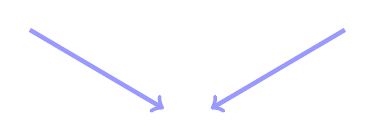
\begin{tikzpicture}
	\draw[ultra thick, color=blue!40!white, ->] (-2,0) -- (-.3,-1); 
	\draw[ultra thick, color=blue!40!white, ->] (2,0) -- (.3,-1); 
\end{tikzpicture}

\begin{tikzpicture}
	[graph,
	 level 1/.style={sibling distance=2cm, level distance=1cm},
	 level 2/.style={sibling distance=2cm, level distance=1cm},
	 level 3/.style={sibling distance=1cm, level distance=1.5cm}]
	 
  \node (a) [knoten] {$a$}
  	child { node (b1) [knoten] {$b$}
  		child { node (c1) [knoten] {$c$}
  			child { node (l1) [blatt] {0} edge from parent node [left] {$\overline{c}$} }
  			child { node (l2) [blatt] {1} edge from parent node [right] {$c$} }
  			edge from parent node [left] {$\overline{b}$}
  		}
  		edge from parent node [left, above] {$a$}
  	}
  	child { node (b2) [knoten] {$b$}
  		child { node (c2) [knoten] {$c$}
  			child { node (l3) [blatt] {1} edge from parent node [left] {$\overline{c}$} }
  			child { node (l4) [blatt] {0} edge from parent node [right] {$c$} }
  			edge from parent node [right] {$b$} 
  		}
  		edge from parent node [right, above] {$\overline{a}$} % right, above could also be realized with xshift=10pt and yshift=10pt
  	};
  	
  	\draw (b1) to node [near start, above] {$b$} (c2);
  	\draw (b2) to node [near start, above] {$\overline{b}$} (c1);
  	
  	\begin{pgfonlayer}{background}
  	\node [rectangle, fill=black!10!white, fit=(c2)(l3)(l4)] {};
  	\node [rectangle, fill=blue!10!white, fit=(c1)(l1)(l2)] {};
	\end{pgfonlayer}
\end{tikzpicture}


\begin{tikzpicture}
	\draw[ultra thick, color=black!40!white, ->] (0,0) -- (0,-1); 
\end{tikzpicture}

\begin{tikzpicture}
	[graph,
	 level 1/.style={sibling distance=2cm, level distance=1cm},
	 level 2/.style={sibling distance=2cm, level distance=1cm},
	 level 3/.style={sibling distance=1cm, level distance=1.5cm}]
	 
  \node (a) [knoten] {$a$}
  	child { node (b1) [knoten] {$b$}
  		child { node (c1) [knoten] {$c$}
  			child { node (l1) [blatt] {0} edge from parent node [left] {$\overline{c}$} }
  			edge from parent node [left] {$\overline{b}$}
  		}
  		edge from parent node [left, above] {$a$}
  	}
  	child { node (b2) [knoten] {$b$}
  		child { node (c2) [knoten] {$c$}
  			child { node (l2) [blatt] {1} edge from parent node [right] {$\overline{c}$} }
  			edge from parent node [right] {$b$} 
  		}
  		edge from parent node [right, above] {$\overline{a}$} % right, above could also be realized with xshift=10pt and yshift=10pt
  	};
  	
  	\draw (b1) to node [near start, above] {$b$} (c2);
  	\draw (b2) to node [near start, above] {$\overline{b}$} (c1);
  	
  	\draw (c1) to node [near start, above] {$c$} (l2);
  	\draw (c2) to node [near start, above] {$c$} (l1);
\end{tikzpicture}
\end{figure}

Führen die beiden ausgehenden Kanten eines Knotens auf denselben Knoten oder dasselbe Blatt so kann der Knoten gelöscht werden und dessen eingehende Kanten auf das Kind des gelöschten Knotens verzweigt werden. 
\begin{figure}[hp]
\centering
\begin{tikzpicture}[graph, bend angle=45]
	\node[] (a) {}
	  child{ node[knoten] (b1) {$b$}
	  	child{ node (c1) {} }
	  	child[missing]{} }
		child{ node[knoten] (b2) {$b$}
	  	child[missing]{}
	  	child{ node (c2) {} } };
	\node[knoten, below=of a, yshift=-1cm] (c) {$c$}
		edge node[right, above, xshift=0.7mm] {$b$} (b1)
		edge node[left, above, xshift=-0.7mm] {$\overline{b}$}(b2);
	\node[blatt, below=of c] {$y$}
		edge[bend left] node[left] {$\overline{c}$} (c)
		edge[bend right] node[right] {$c$} (c);
		
	\begin{scope}[xshift=4cm]
		\node[] (a') {}
		  child{ node[knoten] (b1') {$b$}
		  	child{ node (c1') {} }
		  	child[missing]{} }
			child{ node[knoten] (b2') {$b$}
		  	child[missing]{}
		  	child{ node (c2') {} } };
		\node[blatt, below=of a', yshift=-1cm] (c') {$y$}
			edge node[right, above, xshift=0.7mm] {$b$} (b1')
			edge node[left, above, xshift=-0.7mm] {$\overline{b}$}(b2');
	\end{scope}
	
	\draw[->, ultra thick, color=black!35] (c2) to (c1');
\end{tikzpicture}
\caption{Löschen eines Knotens}
\end{figure}

\section{Quine-McCluskey-Verfahren}
Nach dem Quine-McCluskey-Verfahren können systematisch Terme zusammengefasst werden, welche sich durch Negation einer einzigen Variablen unterscheiden. Das Quine-McCluskey-Verfahren eignet sich im Gegensatz zu KV-Diagrammen für Funktionen mit beliebig vielen Eingangsvariablen. Außerdem ist es leicht zu automatisieren. Beim händischen Minimieren von Funktionen sollten für Funktionen mit 4 oder weniger Eingangsvariablen KV-Diagramme verwendet werden, da diese übersichtlicher und für uns Menschen leichter zu lösen sind. Für Funktionen mit mehr als 4 Eingangsvariablen sollte das Quine-McCluskey-Verfahren eingesetzt werden.

Die Vereinfachung geschieht mittels Ordnungstabellen, welche schrittweise reduziert werden. 
\begin{enumerate}
  \item Die Minterme der Funktion werden aufgrund der Anzahl affirmierter\footnote{Die Affirmation ist das Gegenteil der Negation. Eine affirmierte Variable ist also eine Variable als solche.} Variablen zusammengefasst. So entstehen Gruppen von Termen, wobei alle Terme einer jeweiligen Gruppe gleich viele affirmierte Variablen besitzen. Die so entstandene Ordnung lässt sich in einer Ordnungstabelle notieren, wobei die Gruppen nach Anzahl der affirmierten Variablen aufsteigend sortiert werden.
  \item Anschließend werden jeweils zwei Gruppen zusammengefasst, welche in der Sortierung direkt nebeneinander stehen. Eine Zusammenfassung zweier Terme wird vollzogen, wenn die Terme sich in ausschließlich einer Stelle durch Affirmation und Negation derselben Stelle unterscheiden. Die zusammengefassten Terme werden wiederum neuen Gruppen zugeordnet und in einer Ordnungstabelle nach gleichem Schema notiert. So entstehen Tabellen höherer Ordnung bis keine weitere Zusammenfassung möglich ist.
  \item Terme, welche nicht weiter zusammengefasst werden konnten werden aufgrund dieser Eigenschaft Primimplikanten genannt. Für die minimierte Funktion sind allerdings nicht zwingend alle Primimplikanten notwendig. Primimplikanten, welche für die Funktion notwendig sind, werden Kernimplikanten genannt. Die Kernimplikanten werden anhand der Primimplikantentafel bestimmt. Dabei muss jeder Minterm von mindestens einem Kernimplikanten abgedeckt sein. Es gilt also eine minimale Anzahl an Kernimplikanten zu bestimmen, wobei jeder Minterm über die Menge der ausgewählten Kernimplikanten abgedeckt sein muss.
\end{enumerate}

Beispiel: Die Funktion f mit den vier Eingangsvariablen $a$, $b$, $c$ und $d$ sei durch ihre Minterme $\{m_i \mid i \in {0,2,5,8,10,12,13,15}\}$ eindeutig bestimmt.
$$ f(a,b,c,d) = \overline{a}\overline{b}\overline{c}\overline{d} + \overline{a}b\overline{c}\overline{d} + a\overline{b}c\overline{d} + \overline{a}\overline{b}\overline{c}d + \overline{a}b\overline{c}d + \overline{a}\overline{b}cd + a\overline{b}cd + abcd$$
\begin{center}
Die Ordnungstabelle 0-ter Ordnung ist:

\begin{tabular}{c *{4}{c} c l}
Term & \multicolumn{4}{c}{Belegung} & Gruppe & Notiz \\
     & $a$ & $b$ & $c$ & $d$        &        &       \\ \hline
 0   & $0$ & $0$ & $0$ & $0$        & 0      &       \\ \hline
 2   & $0$ & $1$ & $0$ & $0$        & 1      &       \\
 8   & $0$ & $0$ & $0$ & $1$        &        &       \\ \hline
 5   & $1$ & $0$ & $1$ & $0$        & 2      &       \\
10   & $0$ & $1$ & $0$ & $1$        &        &       \\
12   & $0$ & $0$ & $1$ & $1$        &        &       \\ \hline
13   & $1$ & $0$ & $1$ & $1$        & 3      &       \\ \hline
15   & $1$ & $1$ & $1$ & $1$        & 4      &       \\
\end{tabular} 
\end{center}

\begin{center}
Die Ordnungstabelle 1-ter Ordnung ist:

\begin{tabular}{c *{4}{c} c l}
Term  & \multicolumn{4}{c}{Belegung} & Gruppe & Notiz \\
      & $a$ & $b$ & $c$ & $d$        &        &       \\ \hline
 0,2  & $0$ & $-$ & $0$ & $0$        & 0      &       \\ 
 0,8  & $0$ & $0$ & $0$ & $-$        &        &       \\ \hline
 2,10 & $0$ & $1$ & $0$ & $-$        & 1      &       \\ 
 8,10 & $0$ & $-$ & $0$ & $1$        &        &       \\
 8,12 & $0$ & $0$ & $-$ & $1$        &        & prim  \\ \hline
 5,13 & $1$ & $0$ & $1$ & $-$        & 2      & prim  \\ 
12,13 & $-$ & $0$ & $1$ & $1$        &        & prim  \\ \hline
13,15 & $1$ & $-$ & $1$ & $1$        & 3      & prim  \\
\end{tabular} 
\end{center}

\begin{center}
Die Ordnungstabelle 2-ter Ordnung ist:

\begin{tabular}{c *{4}{c} c l}
	Term       & \multicolumn{4}{c}{Belegung} & Gruppe & Notiz \\
	~          & a   & b   & c   & d   & ~    & ~              \\ \hline
	$0,2,8,10$ & $-$ & $0$ & $-$ & $0$ & $0$  & prim           \\
	$0,8,2,10$ & $-$ & $0$ & $-$ & $0$ & ~    & streichen      \\
\end{tabular}
\end{center}

\begin{center}
die Primimplikantentafel ist also:
\begin{tabular}{l|*{8}{l|}l}
                & \multicolumn{8}{c|}{Minterme}                       & ~     \\
  Primimplikant & 0    & 2    & 5    & 8    & 10   & 12 & 13   & 15   & ~     \\ \hline
  $8,12$        & ~    & ~    & ~    & + *  & ~    & +  & ~    & ~    & $P_1$ \\
  $5,13$        & ~    & ~    & + \# & ~    & ~    & ~  & + *  & ~    & $K_1$ \\
  $12,13$       & ~    & ~    & ~    & ~    & ~    & +  & + *  & ~    & $P_2$ \\
  $13,15$       & ~    & ~    & ~    & ~    & ~    & ~  & + \# & + \# & $K_2$ \\
  $0,2,8,10$    & + \# & + \# & ~    & + \# & + \# & ~  & ~    & ~    & $K_3$ \\
\end{tabular}
\end{center}
Die Minterme $m_0$, $m_5$, $m_8$, $m_{10}$, $m_{13}$ und $m_{15}$ werden über die Terme $K_1$, $K_2$ und $K_3$ abgedeckt. Wie an der Tafel zu erkennen ist, kann der Minterm $m_{12}$ von $P_1$ oder $P_2$ abgedeckt werden. Daher muss einer der beiden Terme als Kernimplikant gewählt werden. Es gibt also zwei mögliche minimierte Formen der Funktion:
\begin{align*}
	f(a,b,c,d) &= \overline{a}\overline{b}\overline{c}\overline{d} + \overline{a}b\overline{c}\overline{d} 
	              + a\overline{b}c\overline{d} + \overline{a}\overline{b}\overline{c}d + \overline{a}b\overline{c}d 
	              + \overline{a}\overline{b}cd + a\overline{b}cd + abcd \\
	           &= \overline{a}\overline{b}d + a\overline{b}c + acd + \overline{b}\hspace{2pt}\overline{d} \\
	           &= \overline{b}cd + a\overline{b}c + acd + \overline{b}\hspace{2pt}\overline{d} \\
\end{align*}








